\chapter{Fizyczny opis zagadnienia}
\label{cha:model}

% Twierdzenia
\newtheorem{torricelli}{Prawo Torricellego}[chapter]
\newtheorem{mass}{Prawo zachowania masy}[chapter]

Rozważany układ składa się z trzech zbiorników połączonych szeregowo, czy też kaskadowo.
W związku z tym płyn (woda), którym jest napełniony pierwszy zbiornik, przepływa przez otwór o zadanym oporze wypływu do drugiego zbiornika.
Stamtąd wypływa przez drugi otwór o zadanym oporze do trzeciego zbiornika, skąd przez kolejny taki otwór wypływa do zewnętrznego naczynia.
Z niego woda jest pompowana z powrotem do pierwszego zbiornika.
Całość układu jest przedstawiona schematycznie na rys. \ref{fig:zbiorniki}.


\begin{figure}[hpt]
	\centering
	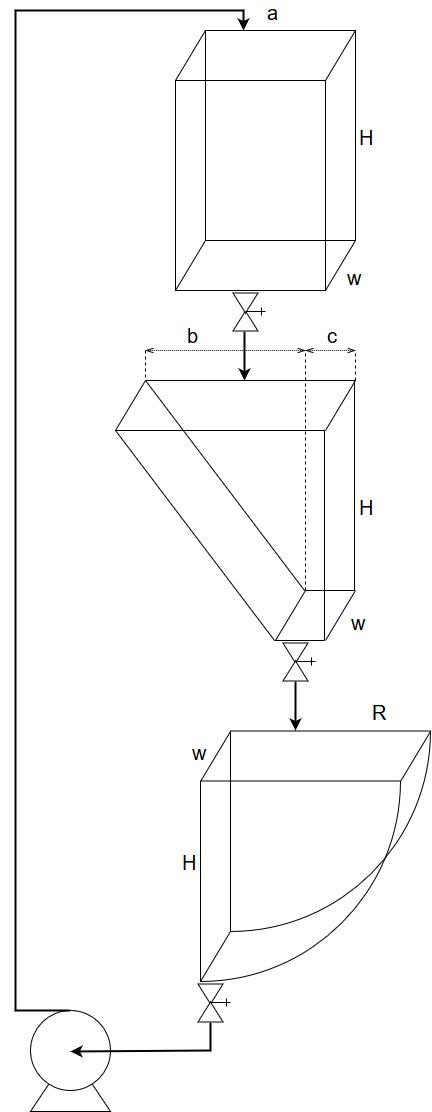
\includegraphics[scale=.5]{Grafika/schemat_zbiornikow}
	\caption{Układ zbiorników z zaznaczonymi wymiarami. Źródło: własne.}\label{fig:zbiorniki}
\end{figure}

\section{Wprowadzenie z zakresu dynamiki płynów}
\label{sec:plyny}

W niniejszym podrozdziale zostały przypomniane podstawowe prawa fizyki związane z przepływem cieczy oraz jego związkiem z poziomem tej cieczy w zbiorniku.

%-------------------------------------------------
\subsection{Równanie Bernoulliego i prawo Torricellego}
\label{sub:plyny-torr}

Równanie Bernoulliego jest jednym z podstawowych praw termodynamiki płynów idealnych. Mówi ono, że wzrost prędkości przepływu cieczy musi wiązać się ze spadkiem ciśnienia lub energii potencjalnej.
Ma kilka postaci; najpopularniejszą jest tzw. szczególne równanie Bernoulliego, które wiąże energię mechaniczną płynu z jego prędkością w danym miejscu, wysokością w układzie odniesienia służącym do wyznaczania energii potencjalnej, ciśnieniem i gęstością.
W takiej formie można je stosować tylko do cieczy nieściśliwych i nielepkich, jednocześnie zakładając stacjonarność i bezwirowość przepływu.

Ta szczególna postać równania Bernoulliego jest przedstawiona jako równanie \ref{eq:bernoulli}.

\begin{equation}\label{eq:bernoulli}
e_{m} = \frac{v^2}{2} + gh + \frac{p}{\rho} = const
\end{equation}

Oznaczenia:
\begin{itemize}
	\item $e_{m}$ - energia jednostki masy cieczy,
	\item $v$ - prędkość cieczy w danym miejscu,
	\item $g$ - przyspieszenie grawitacyjne,
	\item $h$ - wysokość w układzie odniesienia, w którym jest wyznaczana energia potencjalna,
	\item $p$ - ciśnienie cieczy w danym miejscu,
	\item $\rho$ - gęstość cieczy.
\end{itemize}

Z równania Bernoulliego można wyprowadzić bezpośrednią zależność między prędkością cieczy a jej poziomem w zbiorniku. Jest ona znana pod nazwą prawa Torricellego i przedstawiona jako równanie \ref{eq:torricelli} (przyjęto oznaczenia takie jak w przypadku równania \ref{eq:bernoulli}).
Można owo prawo zapisać w bardziej ogólnej formie słownej:

\begin{torricelli}
    Prędkość wypływu cieczy jest proporcjonalna do pierwiastka kwadratowego z poziomu cieczy w zbiorniku.
    \begin{equation}\label{eq:torricelli}
    v = \sqrt{2gh}
    \end{equation}
\end{torricelli}
Takie sformułowanie tego prawa będzie istotne w dalszych krokach wyznaczania modelu matematycznego rozważanego układu.


\subsection{Bilans masy}
\label{sub:plyny-bilans}

Kolejnym zjawiskiem fizycznym, którego zrozumienie jest potrzebne, aby wyznaczyć model matematyczny rozważanego w niniejszej pracy układu zbiorników, jest bilans masy, czyli bezpośrednia konsekwencja \emph{prawa zachowania masy}.

\begin{mass}
    Masa układu ciał (suma mas wszystkich ciał wchodzących w skład tego układu) nie zmienia się podczas przemian i oddziaływań fizycznych w nim zachodzących.
    \begin{equation}\label{eq:mass-conservation}
        m_{uk} = const
    \end{equation}
\end{mass}

Rozważając układ pojedynczego zbiornika z cieczą, do którego ta ciecz jest nalewana i z którego się ona wylewa, można sformułować następstwo tego prawa dane równaniem \ref{eq:mass-balance}. Mówi ono, że zmiana masy w rozważanym zbiorniku - $m_{zb}$ - jest równa zmianie masy do niego wpływającej - $m_{we}$ - i wypływającej - $m_{wy}$.

\begin{equation}\label{eq:mass-balance}
    \frac{\partial m_{we}}{\partial t} - \frac{\partial m_{wy}}{\partial t} =\frac{\partial m_{zb}}{\partial t}
\end{equation}

Przyjmując założenie, że ciecz w zbiorniku i poza nim ma stałą gęstość $\rho$ oraz stosując następujące podstawienia:
\begin{itemize}
    \item $m_{zb} = V_{zb}\cdot\rho$, gdzie $V_{zb}$ to objętość cieczy w zbiorniku,
    \item $V_{zb} = A_{zb} \cdot h_{zb}$, gdzie $A_{zb}$ to pole przekroju poprzecznego zbiornika, a $h_{zb}$ to wysokość słupa cieczy w tym zbiorniku
\end{itemize}
można przedstawić powyższą zależność w postaci opisanej zależnością \ref{eq:tank-mass-balance} (za: \cite{Postlethwaite}).

\begin{equation}\label{eq:tank-mass-balance}
    A_{zb} \cdot \frac{\partial h_{zb}}{\partial t} = \frac{\partial V_{we}}{\partial t} - \frac{\partial V_{wy}}{\partial t}
\end{equation}

Strumień (zmiana objętości cieczy w czasie) wypływający z takiego zbiornika można otrzymać na podstawie prawa Torricellego - jest on dany zależnością \ref{eq:tank-outflow}, gdzie $C$ to stała proporcjonalności wypływu. W rozważanym układzie będzie on zależeć od ustawienia zaworu wyjściowego z danego zbiornika, a więc można powiedzieć, że strumień opisuje opór wypływu ze zbiornika (za: \cite{TanksManual}).

\begin{equation}\label{eq:tank-outflow}
\frac{\partial V_{wy}}{\partial t} = C\cdot\sqrt{h_{zb}}
\end{equation}

Jeśli chodzi o strumień wpływający, to dla drugiego i trzeciego zbiornika jest on równy strumieniowi wypływającemu z poprzedniego zbiornika. Można przyjąć, że dla pierwszego zbiornika ten strumień to sterowanie pompą. Będzie ono oznaczone symbolem $u$.

Pola powierzchni przekrojów poprzecznych wszystkich trzech zbiorników przedstawiono jako równanie \ref{eq:model-fields}. Zastosowano oznaczenia z \ref{fig:zbiorniki}.

\begin{equation}\label{eq:model-fields}
    \begin{array}{lr}
        A_{1} = w \cdot a \\
        A_{2} = c\cdot w + \frac{h_{2}}{h_{max}}\cdot b\cdot w \\
        A_{3} = w\cdot \sqrt{R^{2} - (R - h_{3})^{2}}
    \end{array}
\end{equation}

%-------------------------------------------------
\subsection{Rodzaje przepływów}
\label{sub:plyny-przeplywy}

Przytoczona wcześniej szczególna postać równania Bernoulliego (równanie \ref{eq:bernoulli}) jest obwarowana założeniem stacjonarności przepływu. Oznacza to dwie rzeczy:
\begin{enumerate}
    \item Wartości wektorów prędkości cieczy są stałe w czasie.
    \item Poszczególne ,,warstwy'' cieczy nie wpływają na siebie.
\end{enumerate}

Drugi z tych warunków jest znany pod nazwą przepływu laminarnego, który zwykle ma miejsce przy niskich prędkościach cieczy. W takim typie przepływu nie występują żadne jego zaburzenia (ruchy wirowe, prądy przeciwne itp.), a zachowanie poszczególnych ,,warstw'' cieczy porównać można do tasowania kart: przepływają obok siebie bez wpływania jedna na drugą. Jej cząstki będące blisko powierzchni przemieszczają się po liniach równoległych do tafli cieczy.

Niestety, w rzeczywistości ciężko jest spełnić założenie laminarności przepływu, nie mówiąc już o jego stacjonarności. W związku z tym można zastosować pewne praktyczne uogólnienie zależności \ref{eq:tank-outflow} w stosunku do cieczy wypływających w sposób nielaminarny. Polega ono na zastąpieniu pierwiastka we wspomnianym wzorze parametrem $\alpha$, którego wartość można dobrać na podstawie pomiarów w rzeczywistym układzie (przykład podany w \cite{TanksManual}). Uwzględniają to uogólnienie, można zapisać nowe sformułowanie zależności \ref{eq:tank-outflow} jako równanie \ref{eq:tank-outflow-nonlmnr}.

\begin{equation}\label{eq:tank-outflow-nonlmnr}
    \frac{\partial V_{wy}}{\partial t} = C\cdot h_{zb}^{\alpha}
\end{equation}


\section{Model matematyczny zestawu zbiorników}
\label{sec:model}

Na podstawie podanych wcześniej zależności można zdefiniować model matematyczny rozważanego układu zbiorników.
Jest on dany równaniem \ref{eq:model} (za: \cite{TanksManual}).

\begin{equation}\label{eq:model}
\left \{
\begin{array}{lr}
\frac{\partial h_{1}}{\partial t} = \frac{u - C_{1}{h_{1}}^{\alpha_{1}}}{aw} \\[8pt]
\frac{\partial h_{2}}{\partial t} = \frac{C_{1}{h_{1}}^{\alpha_{1}} -  C_{2}{h_{2}}^{\alpha_{2}}}{cw + \frac{h_{2}}{h_{max}}bw} \\[12pt]
\frac{\partial h_{3}}{\partial t} = \frac{C_{2}{h_{2}}^{\alpha_{2}} -  C_{3}{h_{3}}^{\alpha_{3}}}{w\sqrt{R^{2} - (R - h_{3})^{2}}}
\end{array}
\right.
\end{equation}

Oznaczenia:
\begin{itemize}
    \item $h(t) = [h_{1}(t)~ h_{2}(t)~ h_{3}(t)]^{T}$ - poziomy wody w zbiornikach,
    \item $u(t)$ - sterowanie pompą,
    \item $a$ - szerokość pierwszego zbiornika,
    \item $b$ - szerokość trójkątnej części drugiego zbiornika,
    \item $c$ - szerokość prostopadłościennej części drugiego zbiornika,
    \item $R$ - promień trzeciego zbiornika,
    \item $w$ - głębokość zbiorników,
    \item $h_{max}$ maksymalna wysokość słupa wody w zbiornikach,
    \item $C_{i}$ - opór wypływu z $i$-tego zbiornika,
    \item $\alpha_{i}$ - współczynnik wypływu z $i$-tego zbiornika.
\end{itemize}

Wszystkie wymiary w powyższym wzorze zostały przedstawione na rys. \ref{fig:zbiorniki}. Są na nim również oznaczone opory wypływów $C_{1}$ - $C_{3}$ przy odpowiednich zaworach.

Przyjmując $\alpha_{i} = \frac{1}{2}, \forall_{i \in \{1, 2, 3\}}$, można uszczegółowić powyższy model, zakładając tylko przepływ laminarny.
Taka właśnie jego postać będzie wykorzystywana przy analitycznym wyznaczeniu współczynników równania sprzężonego (definicja znajduje się w sekcji \ref{sub:toc-def-intro}), które jest przeprowadzone w podrozdziale \ref{sub:toc-ctrl}.
W rzeczywistości, jak zostało wspomniane w podrozdziale \ref{sub:plyny-przeplywy}, wartości tych współczynników będą musiały być trochę mniejsze, aby oddać faktyczny sposób przepływu wody między zbiornikami.

W rozważanym układzie zbiorników przyjmuje się następujące ograniczenia (pomijając oczywiste $t \geq 0$):
\begin{itemize}
    \item ograniczenia równościowe:
    \begin{equation}\label{eq:model-eq-const}
    \begin{array}{lr}
        h_{1}(0) = h_{10}\\
        h_{2}(0) = h_{20}\\
        h_{3}(0) = h_{30}\\
    \end{array}
    \end{equation}
    \item ograniczenia nierównościowe:
    \begin{equation}\label{eq:model-noneq-const}
    \begin{array}{lr}
        \forall_{t \in [0, T]}:~ 0 \leq h_{1}(t) \leq h_{max}\\
        \forall_{t \in [0, T]}:~ 0 \leq h_{2}(t) \leq h_{max}\\
        \forall_{t \in [0, T]}:~ 0 \leq h_{3}(t) \leq h_{max}\\
        \forall_{t \in [0, T]}:~ 0 \leq u(t) \leq u_{max}
    \end{array}
    \end{equation}
\end{itemize}
Parametry $h_{10}$, $h_{20}$ i $h_{30}$ oraz $h_{max}$ traktuje się jako zadane.

Punkty równowagi (nazywane również stanami ustalonymi) takiego systemu będą opisane przez zależność \ref{eq:steady-state-def-model} i wyznaczone przez parę wektora wartości zmiennych stanu $h_{r}$ oraz sterowania $u_{r}$. Brak zależności od czasu owej pary został odpowiednio odnotowany.

\begin{equation}\label{eq:steady-state-def-model}
\frac{\partial h(t)}{\partial t} = 0 ~\Rightarrow~ 
\left \{
\begin{array}{lr}
    \frac{\partial h_{1}}{\partial t} = 0 \\
    \frac{\partial h_{2}}{\partial t} = 0 \\
    \frac{\partial h_{3}}{\partial t} = 0
\end{array}
\right.
\end{equation}

Dla rozważanego układu zbiorników będą miały postać daną zależnością \ref{eq:model-steady-state}.

\begin{equation}\label{eq:model-steady-state}
\begin{array}{lr}
u_{r} = C_{1}h_{1}^{\alpha_{1}} = C_{2}h_{2}^{\alpha_{2}} = C_{3}h_{3}^{\alpha_{3}}\\
h_{r} = \begin{bmatrix}
h_{1r}\\h_{2r}\\h_{3r}
\end{bmatrix}
=
\begin{bmatrix}
\big( \frac{\textstyle u_{r}}{\textstyle C_{1}}\big)^{\frac{\scriptstyle 1}{\scriptstyle \alpha_{1}}}\\
\big( \frac{\textstyle u_{r}}{\textstyle C_{2}}\big)^{\frac{\scriptstyle 1}{\scriptstyle \alpha_{2}}}\\
\big( \frac{\textstyle u_{r}}{\textstyle C_{3}}\big)^{\frac{\scriptstyle 1}{\scriptstyle \alpha_{3}}}
\end{bmatrix}
\end{array}
\end{equation}

Wynika z tego, że układ otwarty jest asymptotycznie stabilny, gdyż posiada tylko jeden, zerowy punkt równowagi (pokazany jako wzór \ref{eq:model-zero-state}). Jest to również zgodne z fizyczną naturą tego systemu zbiorników: przy braku zasilania go pompą, cała woda wycieknie ze wszystkich trzech zbiorników.

\begin{equation}\label{eq:model-zero-state}
h_{r}^{0} = \begin{bmatrix}
h_{1r}^{0}\\h_{2r}^{0}\\h_{3r}^{0}
\end{bmatrix} = 
\begin{bmatrix}
0\\0\\0
\end{bmatrix}
\end{equation}

